% chapter 4
% Last edit: 2017-4-27
\chapter{Continuous Random Variables and Probability Distributions}
\section{Probability Density Functions}
\begin{exmp}
Study the ecology of a lake, measure the depth of the lake. Denote $L_{max}$ as the largest depth of the lake.
\[X = \text{depth of the lake}\]
The support of $X$ is $(0, L_{max}]$ \\
This is a continues r.v., but it shares some properties of a discrete r.v.
\end{exmp}

\begin{defn}
In general, X is supported on $[a,b]$ . There is a $f(x)$ satisfying
\begin{enumerate}
\item $f(x) \geq 0, \qquad \forall x \in [a,b]$
\item $\int _a^b f(x) dx=1$
\item $P(c<x<d)=\int _c^d f(x)dx$
\end{enumerate}
Such an $f$ is called the \textbf{probability distribution function(p.d.f)} of $X$
\[f(x)=\lim_{h \to 0} \frac{P(x \leq X \leq x+h)}{h} \]
\end{defn}

\begin{exmp}
X=waiting time of a MTR at Kowloon Tong Station is 
\[f(x)=\begin{cases}
\frac{1}{15}, 	&0 \leq x \leq 15\\
0. &\text{otherwise}
\end{cases}\]
Check
\[\int_0^{15} f(x)dx=\int_0^{15} \frac{1}{15}dx=1\]
\[P(5\leq X \leq 10)=\int_5^{10} \frac{1}{15}dx=\frac{1}{3}\]
"uniform r.v"
\end{exmp}


\section{Cumulative Distribution Functions and Expected Values}
\subsection{The Cumulative Distribution Function}
\begin{defn}
Let $X$ be a constant r.v. with c.d.f $f(x)$. Its \textbf{c.d.f.} is 
\[F(x)=P(X \leq x)=\int_{-\infty}^{x}f(y)dy\]
\end{defn}

\begin{exmp}
\[X \sim unif(a,b)\]
\[f(x)=\begin{cases}
\frac{1}{b-a}, 	&a \leq x \leq b\\
0. &\text{otherwise}
\end{cases}\]
\[F(x)=\int_{-\infty}^{x}f(y)dy=\begin{cases}
0,		&\text{if } x < a \\
\frac{x-a}{b-a}, 	&a \leq x \leq b\\
1. 		&\text{if } x > b 
\end{cases}\]
\end{exmp}

\begin{exmp}
$X \sim exp(\lambda)$,"exponential r.v"
\[f(x)=\begin{cases}
\lambda e^{-\lambda x}, 	& x >0\\
0. &\text{otherwise}
\end{cases}\]
\[F(x)=\int_{-\infty}^{x}f(y)dy=\begin{cases}
0,		&\text{if } x < 0 \\
1-e^{-\lambda x}. 		&\text{if } x \geq 0
\end{cases}\]
If $x>0$,
\begin{align*}
\int_{-\infty}^{x}f(y)dy= & \int_{0}^{x}\lambda e^{-\lambda y}dy=\int_{0}^{x}e^{-\lambda y}d(\lambda y)\\
= & \left.-e^{-\lambda y}\right|_0^x =1-e^{-\lambda x}
\end{align*}
\end{exmp}

\begin{prop}
If X is continuous. For any constant $c$,
\[P(X=c)=0\]
Furthermore, for any $a,b$, we have
\[P(a \leq X \leq b)=P(a <X\leq b)=P(a \leq X< b)=P(a <X< b)\]
\end{prop}



\subsection{Using $F(x)$ to Compute Probabilities}
Let $X$ be a constant r.v. with p.d.f $f(x)$ and c.d.f. $F(x)$,Then
\begin{align*}
&P(X>a)=1-P(X\leq a)=1-F(a)\\
&P(X \geq a)=1-F(a)	\\
&P(a < X <b)=1-F(b)	\\
&P(a<X<b)=P(x<b)-P(x<b)=F(b)-F(a)
\end{align*}

\begin{exmp}
X has a p.d.f 
\[f(x)=\begin{cases}
\frac{1}{8}+\frac{3}{8}x, &\text{if } 0\leq x\leq 2\\
0&\text{otherwise}\\
\end{cases}\]
\[F(x)\int_{-\infty}^{x}f(y)dy=\begin{cases}
0,		&\text{if } x<0\\
\frac{x}{8}+\frac{3}{16}x^2, &\text{if } 0\leq x\leq 2\\
1.		&\text{if }x>2\\
\end{cases}\]
\begin{align*}
&P(1\leq X \leq 1.5)=F(1.5)-F(1)=0.297\\
&P(X\geq 1)=1-F(1)=\frac{11}{16}
\end{align*}
\end{exmp}

\subsection{Obtaining $f(x)$ from $F(x)$}
$X$ continues with $f(x)$ and $F(x)$
\[f(x)=F'(x)\]

\begin{exmp}
$X$ continues with $f(x)=1-e^{-\lambda x}, x>0$
\[f(x)=F'(x)= \lambda e^{-\lambda x}, x>0 \]
\end{exmp}

\subsection{Percentiles of a Continuous Distribution}
\begin{exmp}
John's exam score is at the 85th percentile of the class, meaning that John's score is higher than 85\% of the class.
\end{exmp}

\begin{defn}
Let $0 \leq p \leq 1$, the $(100p)$th percentile of the distribution of $X$, denoted by $\eta_p$ is defined as 
\[p=F(\eta_p)\]
Set up the equation $F(\eta_p)=p$, solve for $\eta_p$.
\end{defn}

\begin{exmp}
$X$ has $f(x)=\begin{cases}
2(1-x), & 0\leq x\leq 1\\
0.		&\text{o.w.}\\
\end{cases}$
\[F(x)=\begin{cases}
0,		&\text{if } x<0\\
2x-x^2, &\text{if } 0\leq x\leq 1\\
1.		&\text{if  }x>1\\
\end{cases}\]
To get 90\% percentile
\[F(\eta_{0.9})=0.9\]
Solve the equation, $\eta_{0.9}=1 \pm \sqrt{0.1}$. Since $0 \leq \eta_{0.9} \leq 1$
\[\eta_{0.9}=1 - \sqrt{0.1}\]
To get 50th percentile, $F(\eta_{0.5})=0.5$
\[\eta_{0.5}=1-\frac{\sqrt{2}}{2}\]
\end{exmp}

\textbf{Median} is the 50th percentile of the distribution of $X$.
\subsection{Mean and Variance}
\begin{defn}
$X$ is continues with $f(x)$ and $F(x)$. The expected or mean value of a continuous rv $X$ with pdf $f(x)$ is
\[E(X)=\int_{-\infty}^{\infty}xf(x)dx \]
\end{defn}

\begin{exmp}
\[f(x)=\begin{cases}
\frac{2}{3}(1-x^2), &\text{if } 0\leq x\leq 1\\
0.		&\text{otherwise}\\
\end{cases}\]
\[E(X)=\int_{-\infty}^{\infty}xf(x)dx=\frac{3}{8} \]
\end{exmp}

\begin{prop}
$X$ is continues with $f(x)$, for any $h(x)$
\[E(h(X))=\int_{-\infty}^{\infty}h(x)f(x)dx\]
Particularly,
\[h(x)=ax+b \qquad E(aX+b)=aE(X)+b\]
\end{prop}

\begin{exmp}
$X \sim uniform(0,1)$
\[f(x)=\begin{cases}
1, &\text{if } 0 \leq x\leq 1\\
0. & \text{if o.w.}
\end{cases}\]
\[h(x)=max\{x,1-x\}\]
\[E[h(x)]=\int_o^1 h(x)f(x)dx\]
\[E(2X+3)=4 \qquad E(X)=\frac{1}{2}\]
\end{exmp}


\begin{defn}
The \textbf{variance} of a continuous random variable $X$ with pdf $f(x)$ and mean value $\mu$ is
\[Var(X)=\int_{-\infty}^{\infty} (x-\mu)^2f(x)dx=E[(X-\mu)^2]\]
\end{defn}

\begin{prop}
\[Var(X)=E[(X-E(X))^2]=E(X^2)-(E(X))^2\]
\end{prop}

\section{The Normal Distribution}
X has p.d.f 
\[f(x)=\frac{1}{\sqrt{2 \pi \sigma^2}} e^{-\frac{(x-\mu)^2}{2 \sigma^2}}   \qquad -\infty< x< \infty \]
Then X has a normal distribution, or $X \sim N(\mu,\sigma^2)$


\begin{figure}[H]
\centering
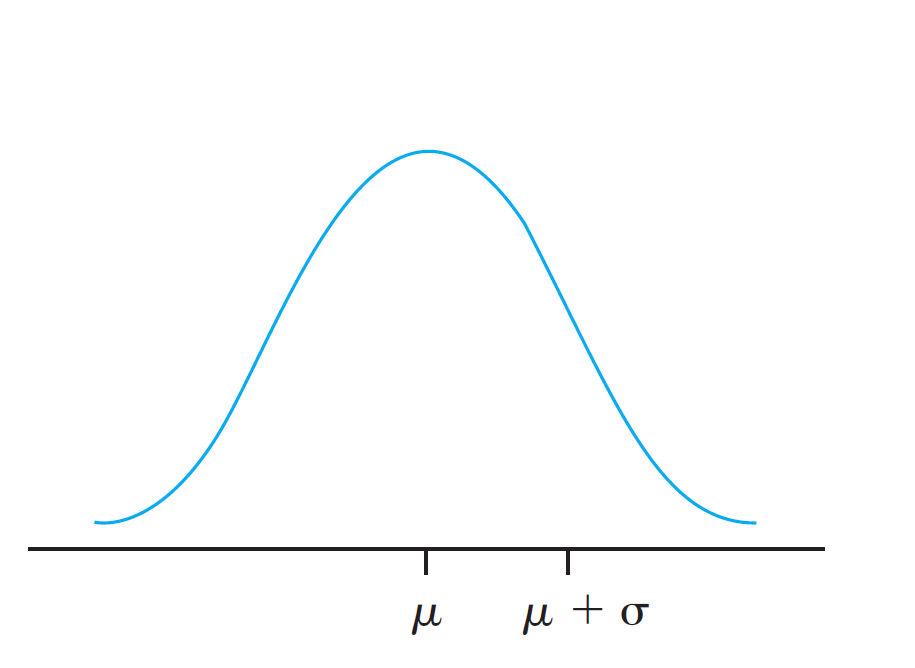
\includegraphics[scale=0.4]{figures/normal_distribution.png}
\caption{Bell-shaped curve}
\end{figure}
Symmetric about $\mu$, $\mu$=shift, $\sigma$=scale, large $\sigma\Rightarrow$large spread out.
 
\begin{prop}
Properties
\begin{enumerate}
\item $E(X)=\mu \qquad	Var(X)=\sigma^2$
\item $f(x) \to 0$, when $x \to \pm \infty$
\end{enumerate}
\end{prop}

\subsection{The Standard Normal Distribution}
The Standard Normal Distribution, $N(0,1)$, denoted by $Z$,
\[f(x)=\frac{1}{\sqrt{2 \pi}} e^{-\frac{x^2}{2}}  \qquad -\infty< x< \infty\]
c.d.f of $Z$
\[\Phi(x)=\int_{-\infty}^{\infty} \frac{1}{\sqrt{2 \pi}} e^{-\frac{x^2}{2}}  dx\]
\begin{align*}
&\Phi(0)=0.5 \\
&\Phi(1.645)=0.95 \qquad \Phi(1.96)=0.975 \\
&\Phi(-1.645)=0.05 \qquad \Phi(-1.96)=0.025
\end{align*}

\begin{exmp}
(1)
\begin{align*}
&P(-1.645 \leq Z \leq 1.96)\\
=&P(Z \leq 1.96)-P(Z \geq -1.645) \\
=&\Phi(1.96)-\Phi(-1.645)=0.975-0.05=0.925
\end{align*}

(2)
\begin{align*}
&P(-0.38 \leq Z \leq 1.25)\\
=&\Phi(1.25)-\Phi(-0.38)=0.8944-(1-\Phi(0.38))\\
=&0.8944-(1-0.6486)=0.5424
\end{align*}
\end{exmp}

\subsubsection{Using Standard Normal Table}

\subsection{Percentiles of the Standard Normal Distribution}
$100p$ th percentile $\eta_{p}$ of $X$ is the solution of 
\[F(\eta_p)=p\]

\begin{exmp}
For $Z$
\[\eta_{0.975}=1.96 \qquad \eta_{0.95}=1.645\]
\[\eta_{0.025}=-1.96 \qquad \eta_{0.05}=-1.645\]
\[\eta_{0.9}=1.28\]
\end{exmp}


\subsection{$z_{\alpha}$ Notation for $z$ Critical Values}
$z_{\alpha}$ will denote the value on the $z$ axis for which $\alpha$ of the area under the $z$ curve lies to the right of $z$. 
\[z_{0.05}=\eta_{0.95}=1.645\]
(lower percentile)
\subsection{Nonstandard Normal Distributions}
If $X \sim N(\mu,\sigma^2) $,then
\[Z=\frac{X-\mu}{\sigma} \sim N(0,1)\]
\begin{align*}
P(a\leq X\leq b) &= P \left(\frac{a-\mu}{\sigma} \leq \frac{X-\mu}{\sigma} \leq \frac{b-\mu}{\sigma} \right)  \\
& = P \left( \frac{a-\mu}{\sigma} \leq Z \leq \frac{b-\mu}{\sigma} \right) =\Phi \left(\frac{b-\mu}{\sigma} \right)- \Phi \left(\frac{a-\mu}{\sigma} \right)
\end{align*}
Similarly,
\begin{align*}
P(X\leq a) &= P \left(\frac{X-\mu}{\sigma} \leq \frac{a-\mu}{\sigma} \right)  \\
& = P \left(  Z \leq \frac{a-\mu}{\sigma} \right) =\Phi \left(\frac{a-\mu}{\sigma} \right)
\end{align*}
\[P(X \geq b)=1-\Phi \left(\frac{b-\mu}{\sigma} \right)\]

\begin{exmp}
$X \sim N(1.25,0.46)$
\begin{align*}
P(1 \leq X\leq 1.75) &= P \left(\frac{1-1.25}{\sqrt{0.46}} \leq \frac{X-1.25}{\sqrt{0.46}} \leq \frac{1.75-1.25}{\sqrt{0.46}} \right)  \\
& = P \left( -0.369 \leq Z \leq 0.737 \right)\\
&=\Phi \left(0.737 \right)- \Phi \left(-0.369 \right)=\boxed{0.4147}
\end{align*}
\end{exmp}

\subsection{Empirical Rule}
If a population distribution of a r.v is roughly normal. Then
\begin{enumerate}
\item 68\% of the values are within 1 s.d of their mean.
\item 95\% of the values are within 2 s.d of their mean.
\item 99.7\% of the values are within 3 s.d of their mean.
\end{enumerate}
\begin{proof}
\begin{align*}
LHS=&P(\mu-\sigma \leq X \leq \mu+\sigma)=P(-1 \leq\frac{X-\mu}{\sigma}\leq 1)\\
=&\Phi(1)-\Phi(-1)=0.8413-(1-0.8413)=68.26\%
\end{align*}
\end{proof}

\subsection{Percentiles of an Arbitrary Normal Distribution}
If $X\sim N(\mu,\sigma^2)$ c.d.f $F(x)$, (100$p$)th percentile of $X$ is the root of 
\begin{align*}
P=F(\eta_p)=&P(X \leq \eta_p)\\ 
=&P\left(\frac{X-\mu}{\sigma} \leq \frac{\eta_p-\mu}{\sigma} \right)=\Phi\left( \frac{\eta_p-\mu}{\sigma} \right)
\end{align*}
So,$\frac{\eta_p-\mu}{\sigma}$ is the $(100p)$th percentile of $N(0,1)$. Therefore, $(100p)$th percentile of $N(\mu,\sigma^2)$=$\mu+\sigma\times[100p\text{th percentile of }N(0,1)]$

\begin{exmp}
$X \sim N(64,0.78^2)$. Then 99.5 percentile of $X$ is $64+0.78\times 2.58=66$, where 2.58 is the 99.5 percentile of $Z$. 
\end{exmp}

\subsection{Approximating the Binomial Distribution}
If $X \sim Binom(n,p)$. When $n$ is large, and $p$ is not too small or too large, s.t. $np \geq 10, n(1-p) \geq 10$. Then $X \sim N(np,np(1-p))$
\[p(x)=\binom nx p^x (1-p)^{n-x} \qquad x=0,1,\dots,n\]


$X \sim Binom(n,p)$\footnote{$X \sim N(np,np(1-p))$, to avoid significant deviation},
\begin{align*}
P(a \leq X \leq b)&=P(a-0.5 \leq X \leq b+0.5)  \\
P(X \leq a) &= P(X \leq a+0.5)	\\
P(X \geq b) &= P(X \geq b-0.5)
\end{align*}

\begin{exmp}
25\% of all drivers in HK don't have insurance. Randomly select 50 drivers. $X=$ \# of drivers uninsured.

(1)$P(X \leq 10)$ \quad (2)$P(5 \leq X \leq 15)$ \\
First $X\sim Binom(50,0.25) \dot{\sim} N(12.5,12.5\times1.75)$

(1) \begin{align*}
P(X\leq 10) =& P(X \leq 10.5) \\
=& P\left( \frac{X-12.5}{\sqrt{12.5\times1.75}}  \leq   \frac{10.5-12.5}{\sqrt{12.5\times1.75}}\right)=\Phi(-0.653)=0.2578
\end{align*}

(2) \begin{align*}
P(5 \leq X\leq 15) =& P(4.5 \leq X \leq 15.5) \\
=& P\left(\frac{4.5-12.5}{\sqrt{12.5\times1.75}} \leq \frac{X-12.5}{\sqrt{12.5\times1.75}}  \leq   \frac{15.5-12.5}{\sqrt{12.5\times1.75}}\right)	\\
=&\Phi(0.95)-\Phi(-2.61)=0.832
\end{align*}
\end{exmp}

\section{The Exponential and Gamma Distributions}
\subsection{The Gamma Function}
\begin{defn}
\[\Gamma(\alpha)=\int_0^{\infty} x^{\alpha-1}e^{-x} dx\]
\end{defn}

This function has the following properties:
\begin{enumerate}
\item $\Gamma(\alpha)=(\alpha-1)\Gamma(\alpha-1)$
\item $\Gamma(1)=1,\Gamma(2)=1,\Gamma(3)=2$\\
$\Gamma(n)=(n-1)! \qquad n=1,2,\dots$
\item $\Gamma(\frac{1}{2})=\sqrt{\pi}$
\end{enumerate}

\subsection{The Gamma Distribution}
\begin{defn}
X follows a Gamma distribution. $X \sim Gamma(\alpha,\beta)$
\[f(x)=\begin{cases}
\frac{1}{\Gamma(\alpha)} \frac{1}{\beta^{\alpha}} x^{\alpha-1} e^{-x/\beta}, & \text{if} \quad x\geq 0\\
0. & \text{if} \quad x < 0
\end{cases}\]
for $\alpha>0, \beta>0$
\end{defn}

If $\beta=1$, $X \sim Gamma(\alpha,1)$. Standard Gamma distribution.
\[f(x)=\begin{cases}
\frac{1}{\Gamma(\alpha)}  x^{\alpha-1} e^{-x}, & \text{if} \quad x\geq 0\\
0. & \text{if} \quad x < 0
\end{cases}\]

Check
\[\int_{0}^{\infty}\frac{1}{\Gamma(\alpha)}  \frac{1}{\beta^{\alpha}} x^{\alpha-1} e^{-x/\beta} dx=1\]
\begin{align*}
L.H.S.&=\int_{0}^{\infty}\frac{1}{\Gamma(\alpha)}   u^{\alpha-1} e^{-u} du \\
&=\frac{1}{\Gamma(\alpha)} \int_{0}^{\infty} u^{\alpha-1} e^{-u} du=1
\end{align*}

\begin{prop}
If $X\sim Gamma(\alpha,\beta)$, then $E(X)=\alpha\beta$, $Var(X)=\alpha\beta^2$
\begin{proof}
\begin{align*}
E(X)&=\int_{0}^{\infty}x \frac{1}{\Gamma(\alpha)} \frac{1}{\beta^{\alpha}} x^{\alpha-1} e^{-x/\beta} dx = \frac{1}{\Gamma(\alpha)} \int_{0}^{\infty} \frac{1}{\beta^{\alpha}} x^{\alpha} e^{-x/\beta} dx  \\
&=\frac{\beta}{\Gamma(\alpha)} \int_{0}^{\infty} \frac{1}{\beta^{\alpha+1}} x^{\alpha} e^{-x/\beta} dx =  \frac{\beta \Gamma(\alpha+1)}{\Gamma(\alpha)} \int_{0}^{\infty}\frac{1}{\Gamma(\alpha+1)}  \frac{1}{\beta^{\alpha+1}} x^{\alpha} e^{-x/\beta} dx \\
&=\frac{\Gamma(\alpha+1)}{\Gamma(\alpha)}\beta =\alpha\beta
\end{align*}
\end{proof}
\end{prop}

\begin{exmp}
Suppose that the reaction time $X$ of a randomly selected individual to a certain stimulus has a standard Gamma distribution with $\alpha=2$.
\[P(3 \leq X \leq 5)=F(5;2)-F(3;2)\]
Here $F(x;\alpha)$ is the c.d.f of $\Gamma(\alpha,1)$
\[Table A.4=0.960-0.801=0.159\]
\end{exmp}

\begin{prop}
If $X\sim Gamma(\alpha,\beta)$, then $X/\beta \sim Gamma(\alpha,1)$
\[P(X\leq x)=P\left(\frac{X}{\beta} \leq \frac{x}{\beta}\right)=F\left(\frac{x}{\beta};\alpha \right)\]
\end{prop}

\begin{exmp}
The survival time $X$ of a randomly selected male mouse exposed to gamma radiation has Gamma distribution with $\alpha=8$, $\beta=15$. Then
\[E(X)=\alpha\beta =8 \times 15 =120\]
\[Var(X)=\alpha \beta^2 =8 \times 15^2 =1800\]
\begin{align*}
P(60 \leq X \leq 120)&=P\left(\frac{60}{15}\leq\frac{X}{15} \leq\frac{120}{15} \right)=F(8;8)-F(4;8) \\
&=0.547-0.051=0.496
\end{align*}
\end{exmp}

\subsection{Exponential distribution}
If $X\sim exp(\lambda)$,
$f(x)=\begin{cases}
\lambda e^{-\lambda x}, 	& x >0\\
0. &\text{otherwise}
\end{cases}$. Then $X$ has an exponential distribution with parameter $\lambda$.

\begin{prop}
If $X\sim exp(\lambda)$. Then $X \sim Gamma(1,1/\lambda)$
\[E(X)=\lambda \qquad Var(X)=\frac{1}{\lambda^2}\]
\end{prop}

\begin{exmp}
X=response time at some computer terminal. $X \sim exp(\lambda)$. Suppose that the expected reacting time is 5 seconds.
\[E(X)=5 \qquad \frac{1}{\lambda}=5 \Rightarrow \lambda=\frac{1}{5}\]
\[P(X\leq 10)=\int_0^{10} \frac{1}{5} e^{-x/5} dx=\left. e^{-x/5}\right|_{0}^{10}=1-e^{-2}. \]
\end{exmp}


In general, if $X\sim exp(\lambda)$,
\[F(x)=\int_0^{x} \lambda e^{-\lambda y} dy=\left. e^{-\lambda y}\right|_{0}^{x}=1-e^{-\lambda x}\]

\subsubsection{Two applications}
\textbf{(A)}Suppose \# of customers coming in any wait time $\sim Possion(\alpha)$, and \# of customers is non-overlapping intervals are independent. Then
\[X= \text{the elapsed time between the successive customers coming in}\sim exp(\alpha)\]
Why? Let $X_1$=waiting time before the 1st customer coming in. Want to show that $X_1 \sim exp()\lambda$, just need to find $f_{X_1}(x)$. Then we just need to find $F_{X_1}(x)$, as $f_{X_1}(x)=F'_{X_1}(x)$.
\begin{align*}
F_{X_1}(x)&= P(X_1\leq x)=P(\text{at least 1 customer in }(0,x)) \\
&= 1-P(\text{no customer in }(0,x)) \\
&=1-\frac{(\alpha x)^0}{0!}e^{-\alpha x}=1-e^{-\alpha x}
\end{align*}
\[f_{X_1}(x)=F'_{X_1}(x)=\alpha e^{-\alpha x} \qquad x>0\]
\[X_1 \sim exp(\lambda)\]


\textbf{(B)Memoryless property}

Suppose component lifetime $\sim exp(\lambda)$. Putting this component into work, after $t_0$ time, check it and find it is still working. What is the probability that it will last at least another $t$ time?\\
Let $T$ = lifetime of this component $\sim exp(\lambda)$
\begin{align*}
P(T\geq t_0+t|T \geq t_0)&=\frac{P(T\geq t_0+t \cap T \geq t_0)}{P(T \geq t_0)} \\
&=\frac{P(T\geq t_0+t)}{P(T \geq t_0)}=\frac{1-P(T\leq t_0+t)}{1-P(T \leq t_0)} \\
&=\frac{1-(1+e^{-\alpha(t_0+t)})}{1-(1+e^{-\alpha t_0})}=\frac{e^{-\alpha(t_0+t)}}{e^{-\alpha t_0}} \\
&=e^{-\alpha t}
\end{align*}

\subsection{The Chi-Squared Distribution}
Let $\nu$ be an integer, if $X \sim Gamma(\nu,\frac{\nu}{2})$, then we say $X$ has a $\chi^2$-distribution with parameter $\nu$, $X \sim \chi^2 (\nu)$.

It's p.d.f is
\[f(x;\nu)=\begin{cases}
\frac{1}{2^{\nu/2}\Gamma(\nu/2)} x^{\nu/2-1}e^{-x/2} & x>0 \\
0 & o.w.
\end{cases}\]


\begin{prop}
Properties
\begin{enumerate}
\item If $X \sim N(0,1)$, then $X^2 \sim \chi^2 (1)$
\item If $X_1 \sim \chi^2 (n)$, $X_2 \sim \chi^2 (m)$, independently. Then $X_1+X_2 \sim \chi^2 (m+n)$ 
\item If $X_1 \sim N(0,1)$, $X_2 \sim N(0,1)$, independently. Then $X_1+X_2 \sim \chi^2 (2)$ 
\end{enumerate}
\end{prop}

\section{Other Continuous Distributions}
\subsection{The Weibull Distribution}
If $X \sim Weibull(\alpha,\beta)$
\[f(x)=\frac{1}{\beta^{\alpha}}x^{\alpha-1}e^{-(x/\beta)^{\alpha}} \qquad x >0\]
If $\alpha=1$, $X \sim Weibull(1,\beta)$. Then $X \sim exp(\frac{1}{\beta}) $

\begin{figure}[H]
\centering
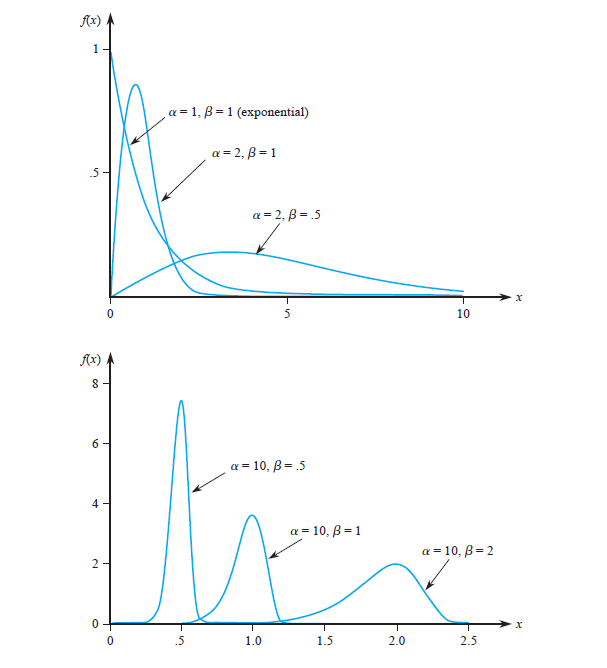
\includegraphics[scale=1]{figures/weibull_distribution.png}
\caption{The Weibull Distribution}
\end{figure}

\begin{prop}
 $X \sim Weibull(\alpha,\beta)$
\begin{enumerate}
\item $E(X)=\beta \Gamma(1+1/\alpha)$
\item $Var(X)=\beta^2\left(\Gamma(1+2/\alpha)-(\Gamma(1+1/\alpha))^2\right)$
\item c.d.f
\[F(x)=\begin{cases}
1-e^{-(\alpha/\beta)^{\alpha}} & x \geq 0 \\
0	&o.w. \\
\end{cases}\]
\end{enumerate}
\end{prop}

\begin{exmp}
$X$ = the strength at  -20 F of a type of steel exhibiting "cold brittleness" at low temperature . $X \sim Weibull(20,100)$

(1) 
\[P(X \leq 105)=F(105)=1-e^{-(105/100)^{20}}=1-0.07=\boxed{0.93}\]
(2)
\[P(90 \leq X \leq 100)=F(110)-F(90)=\left(1-e^{-(110/100)^{20}}\right)-\left(1-e^{-(90/100)^{20}}\right)=\boxed{\dots}\] 
\end{exmp}

\subsection{The Lognormal Distribution}
$X$ is positive. If $\log{X} \sim N(\mu,\sigma^2)$ \footnote{$\log=\ln$} , then $X \sim Lognormal(\mu,\sigma^2)$.
\[f(x)=\frac{1}{\sqrt{2 \pi \sigma^2}} e^{-\frac{(\log{x}-\mu)^2}{2 \sigma^2}}   \qquad  x>0\]
\begin{align*}
E(X)&=e^{\mu +\frac{\sigma^2}{2}} \\
Var(X)&=e^{2\mu +\sigma^2} (e^{\sigma^2}-1)
\end{align*}
\[P(X \leq x)=P(\log{X}\leq \log{x})= P \left(\frac{\log{X}-\mu}{\sigma} \leq \frac{\log{x}-\mu}{\sigma} \right)  =\Phi \left(\frac{\log{x}-\mu}{\sigma} \right)\]

\begin{exmp}
$X$=the modulus of elasticity of some floor system.
\[X \sim Lognormal(0.375,0.25^2)\]
\begin{align*}
E(X)&=e^{0.375+0.25^{2}/2}=1.5\\
Var(X)&= e^{2\times0.375+0.25^{2}}\left(e^{0.25^{2}}-1\right)=0.145\\
P(1 \leq X \leq 2)&=P(\log{1} \leq \log{X}\leq \log{2})\\
&= P \left(\frac{0-0.375}{0.25} \leq \frac{\log{X}-0.375}{0.25} \leq \frac{\log{2}-0.375}{0.25} \right) \\
& =\Phi \left(\frac{\log{2}-0.375}{0.25} \right)-\Phi \left(\frac{-0.375}{0.25} \right)=\boxed{0.8312}
\end{align*}


\end{exmp}

\subsection{The Beta Distribution}
If $X$ has a p.d.f 
\[f(x)=\begin{cases}
\frac{\Gamma(\alpha+\beta)}{\Gamma(\alpha)+\Gamma(\beta)}x^{\alpha-1}(1-x)^{\beta-1}  & 0 \leq x \leq 1 \\
0. & o.w.
\end{cases}\]
Then, $X \sim Beta(\alpha,\beta)$

\begin{prop}
Particularly, if $\alpha=\beta=1$, $X \sim unif(0,1)$
\end{prop}

\begin{prop}
Let $A < B$, and $Y=A+(B-A)X$, then $Y$ be density.
\[f(y)=\begin{cases}
\frac{1}{B-A}\frac{\Gamma(\alpha+\beta)}{\Gamma(\alpha)+\Gamma(\beta)}\left(\frac{y-A}{B-A}\right)^{\alpha-1}\left(\frac{B-y}{B-A}\right)^{\beta-1}  & A \leq x \leq B \\
0. & o.w.
\end{cases}\]
\[Y \sim GBeta\]
\end{prop}

\begin{prop}
If $Y \sim Beta(\alpha,\beta)$
\[E(X)=\frac{\alpha}{\alpha+\beta} \qquad Var(X)=\frac{\alpha\beta}{(\alpha+\beta)(\alpha+\beta+1)}\]
If $Y \sim GBeta(\alpha,\beta,A,B)$
\[E(Y)=A+(B-A)\frac{\alpha}{\alpha+\beta} \qquad Var(Y)=(B-A)^2 \frac{\alpha\beta}{(\alpha+\beta)(\alpha+\beta+1)} \]
Because $Y=A+(B-A)X$, \[E(Y)=E(A+(B-A)X)=A+(B-A)E(X) \qquad Var(Y)=(B-A)^2 Var(X)\]
\end{prop}

\begin{exmp}
\[X=\text{time to complete certain project}\]
\[X \sim GBeta(\alpha=2,\beta=3,A=2,B=5)\]
\[E(X)=2 + (5-2)\frac{2}{2+3}=3.2 \qquad Var(X)=0.36\]
\[P(X \leq 3)=\int_{2}^{3} \frac{1}{5-2}\frac{\Gamma(5)}{\Gamma(2)+\Gamma(3)}\left(\frac{x-2}{3}\right)^{2-1}\left(\frac{5-x}{3}\right)^{3-1} dx=\boxed{0.407}\]
\end{exmp}

\subsection{Challenge Question 2}
Cauchy distribution
\[f(x)=\frac{1}{\pi(1+x^2)}\]
\url{https://en.wikipedia.org/wiki/Cauchy_distribution}